\documentclass{article}
\usepackage[utf8]{inputenc}
\usepackage{pgf-umlcd}

\begin{document}
    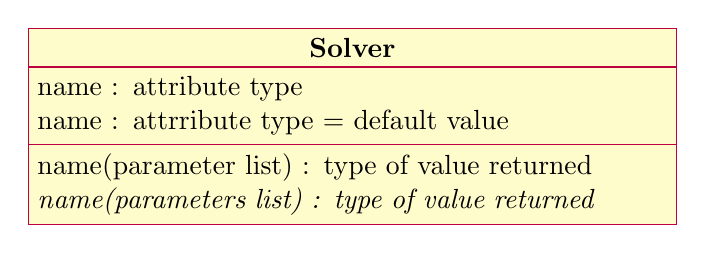
\begin{tikzpicture}
      \begin{class}[text width=8cm]{Solver}{0,0}
        \attribute{name : attribute type}
        \attribute{name : attrribute type = default value}
        \operation{name(parameter list) : type of value returned}
        \operation[0]{name(parameters list) : type of value returned}
      \end{class}
    \end{tikzpicture}

    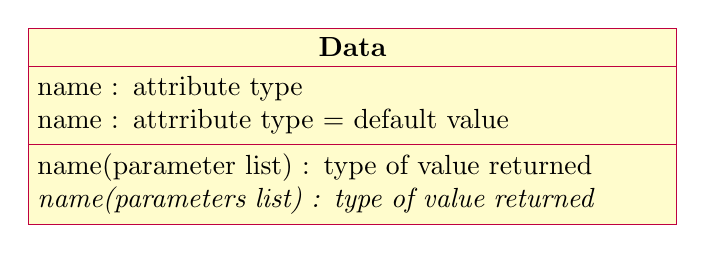
\begin{tikzpicture}
      \begin{class}[text width=8cm]{Data}{0,0}
        \attribute{name : attribute type}
        \attribute{name : attrribute type = default value}
        \operation{name(parameter list) : type of value returned}
        \operation[0]{name(parameters list) : type of value returned}
      \end{class}
    \end{tikzpicture}

    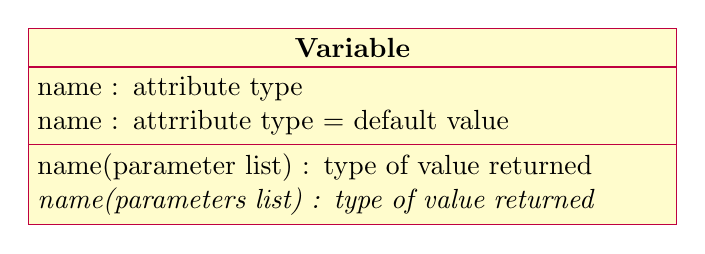
\begin{tikzpicture}
      \begin{class}[text width=8cm]{Variable}{0,0}
        \attribute{name : attribute type}
        \attribute{name : attrribute type = default value}
        \operation{name(parameter list) : type of value returned}
        \operation[0]{name(parameters list) : type of value returned}
      \end{class}
    \end{tikzpicture}

    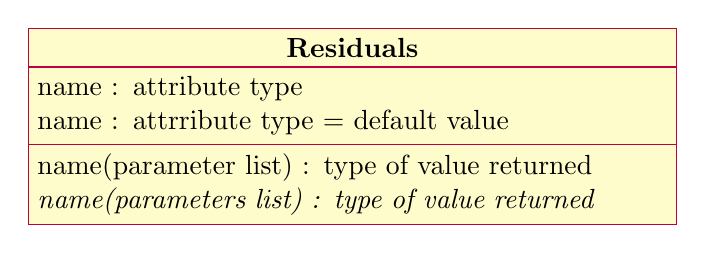
\begin{tikzpicture}
      \begin{class}[text width=8cm]{Residuals}{0,0}
        \attribute{name : attribute type}
        \attribute{name : attrribute type = default value}
        \operation{name(parameter list) : type of value returned}
        \operation[0]{name(parameters list) : type of value returned}
      \end{class}
    \end{tikzpicture}

    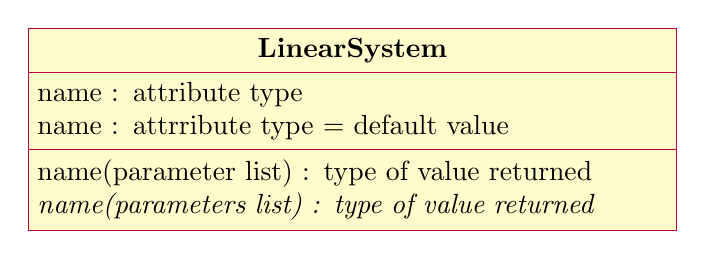
\begin{tikzpicture}
      \begin{class}[text width=8cm]{LinearSystem}{0,0}
        \attribute{name : attribute type}
        \attribute{name : attrribute type = default value}
        \operation{name(parameter list) : type of value returned}
        \operation[0]{name(parameters list) : type of value returned}
      \end{class}
    \end{tikzpicture}

\end{document}
